\documentclass{article}

%package setup
\usepackage{graphicx}
\usepackage{amsmath}
\usepackage{fancyhdr}
\usepackage[margin=1in]{geometry}
\usepackage{comment}
\usepackage{placeins}
\usepackage{parskip}
\usepackage{subcaption}
\usepackage{appendix}
\usepackage{soul}
\usepackage{comment}
\PassOptionsToPackage{hyphens}{url}\usepackage[hidelinks]{hyperref}
\usepackage{matlab-prettifier}
\usepackage{minted}
\usepackage{enumitem}
\usepackage{float}
\usepackage{textcomp, gensymb}
\usepackage{caption}


\pagestyle{fancy}
\fancyhf{} % Clear header/footer settings
\rhead{\thepage} % Page number on the right in the header
\lhead{ASE375 Lab Report 9} % Your lab report title on the left

\begin{document}

\begin{titlepage}
  \centering
  
\includegraphics[width=10cm]{ase-logo-formal.png}  % Adjust the width as needed
  \vspace{1cm}  % Add some vertical space
 
  \Large \textbf{ASE 375 Electromechanical Systems}\\
  \large \textbf{Section 14115}\\
  \vspace{0.5cm}
  \textbf{Monday: 3:00 - 6:00 pm}\\
 
  \vspace{1cm}
 
  \hrule
  \vspace{0.5cm}
 
  \Huge \textbf{Report 9:\\
    Digital Image Correlation}\\
  \Huge \textbf{}\\
 
  \vspace{0.5cm}
  \hrule
 
  \vspace{1cm}
 
  \normalsize \textbf{Andrew Doty, Andres Suniaga, Dennis Hom}\\
  \normalsize \textbf{Due Date: 04/22/2024}
 
\end{titlepage}
\newpage

\tableofcontents
\thispagestyle{empty}
\newpage

\section{Introduction}
In this experiment we investigate the stress concentration around the center holes of (1) an Aluminum and (2) Poly-carbonate test article by using a universal testing machine (UTM) to apply a tensile force to these test materials until failure. Using Digital Image Correlation (DIC) we are able to measure the strain distribution around the center hole of each test article.
\vspace{2.5mm}

This experiment will involve a comparison between our collected stress concentration values and the calculated theoretical values. This lab provides insight into methods used in materials science to determine the strength of materials, such as the stress concentration factor of our Aluminum and Poly-carbonate strips.

\section{Equipment}
Measurement devices and hardware used in this lab include:
\begin{itemize}

\item Instron 3300 Series Universal Testing Machine \hyperlink{1}{[1]} and Bluehill software: 
\vspace{1mm}

Machine used to apply a tensile load to the test articles. Bluehill software used to interface with the testing machine to apply a tensile load to our test articles.
\begin{figure}[H]
    \centering
    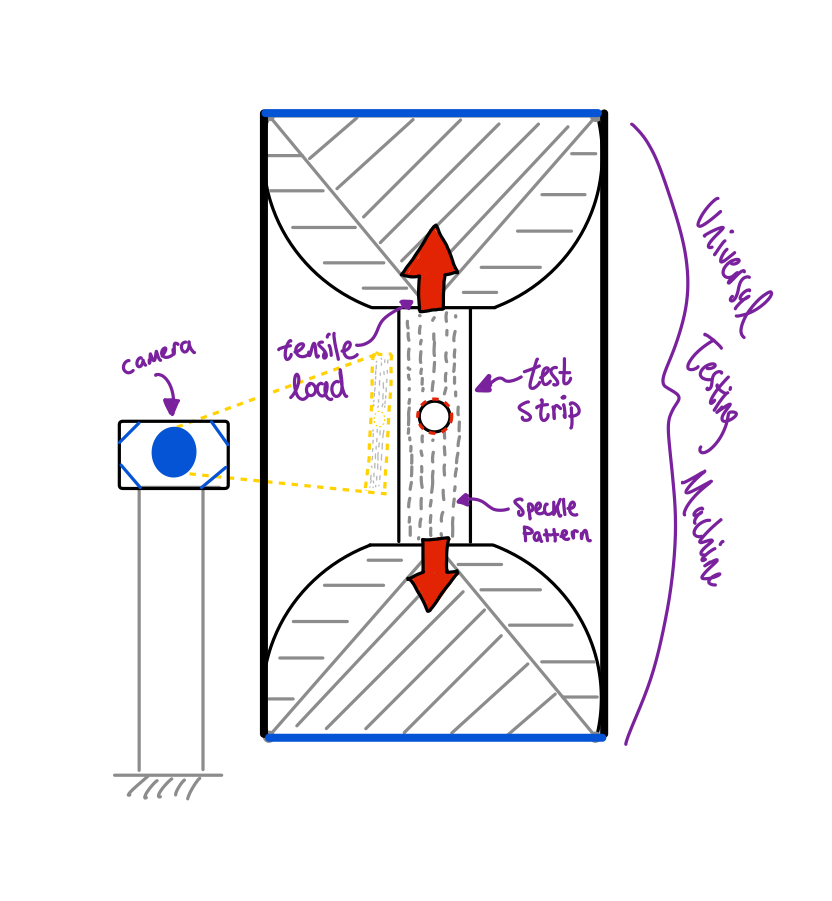
\includegraphics[width = 0.6\textwidth]{lab9images/lab9_emech_setup.png}
    \caption{Experiment Setup}
    \label{fig:setup9}
\end{figure}
\vspace{2.5mm}

\item Digital Calipers, $\epsilon_{b} = 0.005\; \text{mm}$: 
\vspace{1mm}

Used for measuring outer and inner dimensions of objects. In our case we use it to the measure the diameter of the center hole of test articles along with the strips' thickness and width before the experiment.
\vspace{2.5mm}

\item Aluminum and Poly-carbonate Strips:
\vspace{1mm}

Material strips measured in this lab. Used as shown in Figure \ref{fig:setup9}. Material properties of these strips can be found in Table \ref{tab:materialproperties}.

\vspace{2.5mm}

\item Web Camera and Digital Image Correlation Engine (DICe) software \hyperlink{2}{[2]}:
\vspace{1mm}

Used to capture images through a sequence of tensile loads applied to the test articles, as shown in Figure \ref{fig:setup9}. DICe used to analyze strain distribution of the set of images.
\vspace{2.5mm}
\end{itemize}

\section{Procedure}
\subsection{Tensile Loading}
\begin{enumerate}
    \item Before beginning the experiment, measure the thickness, width, and center hole diameter of the test articles with the digital calipers.
    \item Turn on the UTM and open up the Instron Bluehill Software:
    \begin{figure}[H]
        \centering
        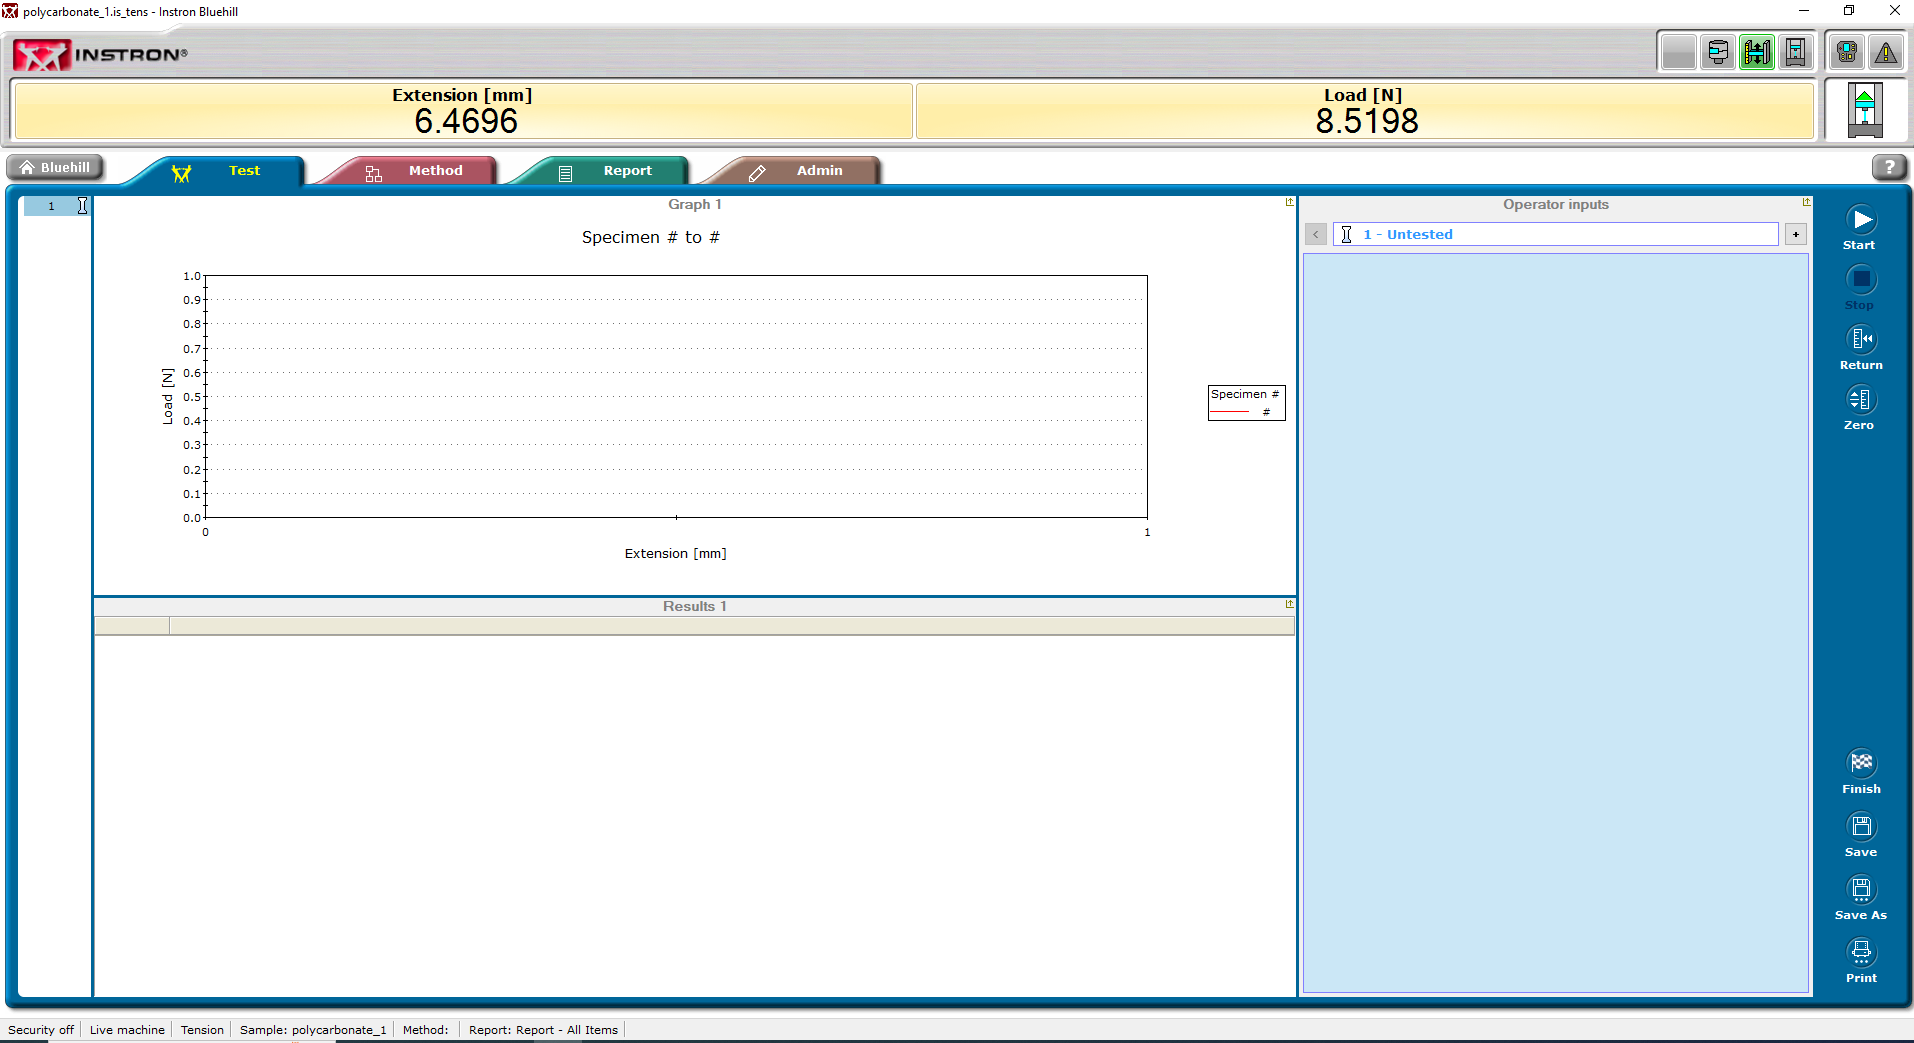
\includegraphics[width = 0.7\textwidth]{lab9images/instrom_bluehill_page.PNG}
        \caption{Bluehill UI}
        \label{fig:bluehill}
    \end{figure}

    Load in the appropriate configuration file for the test articles to the Bluehill software.

    \item Secure one of the test articles within the Instron machine as shown in Figure \ref{fig:setup9}. Ensure that the test article is tightly in place. 

    \item Open the web camera application and ensure the camera is focused on the strip. Once focused, take a snapshot of the strip before loading. Now, begin the loading for the strip in the machine. 
    \begin{itemize}
        \item For Aluminum, take snapshots for every 1000N load (or 1kN)
        \item For Poly-carbonate, take snapshots for every 100N load.
    \end{itemize}

    \item The loading will end once the strips have reached failure. Take a snapshot of the broken strip. 
    \item Save these images. Repeat loading for the other test strip.
    \item Next we will move onto the Digital Image Correlation Process.
\end{enumerate}

\subsection{Digital Image Correlation}
\begin{enumerate}
\item Open up the DICe software:
\begin{figure}[H]
    \centering
    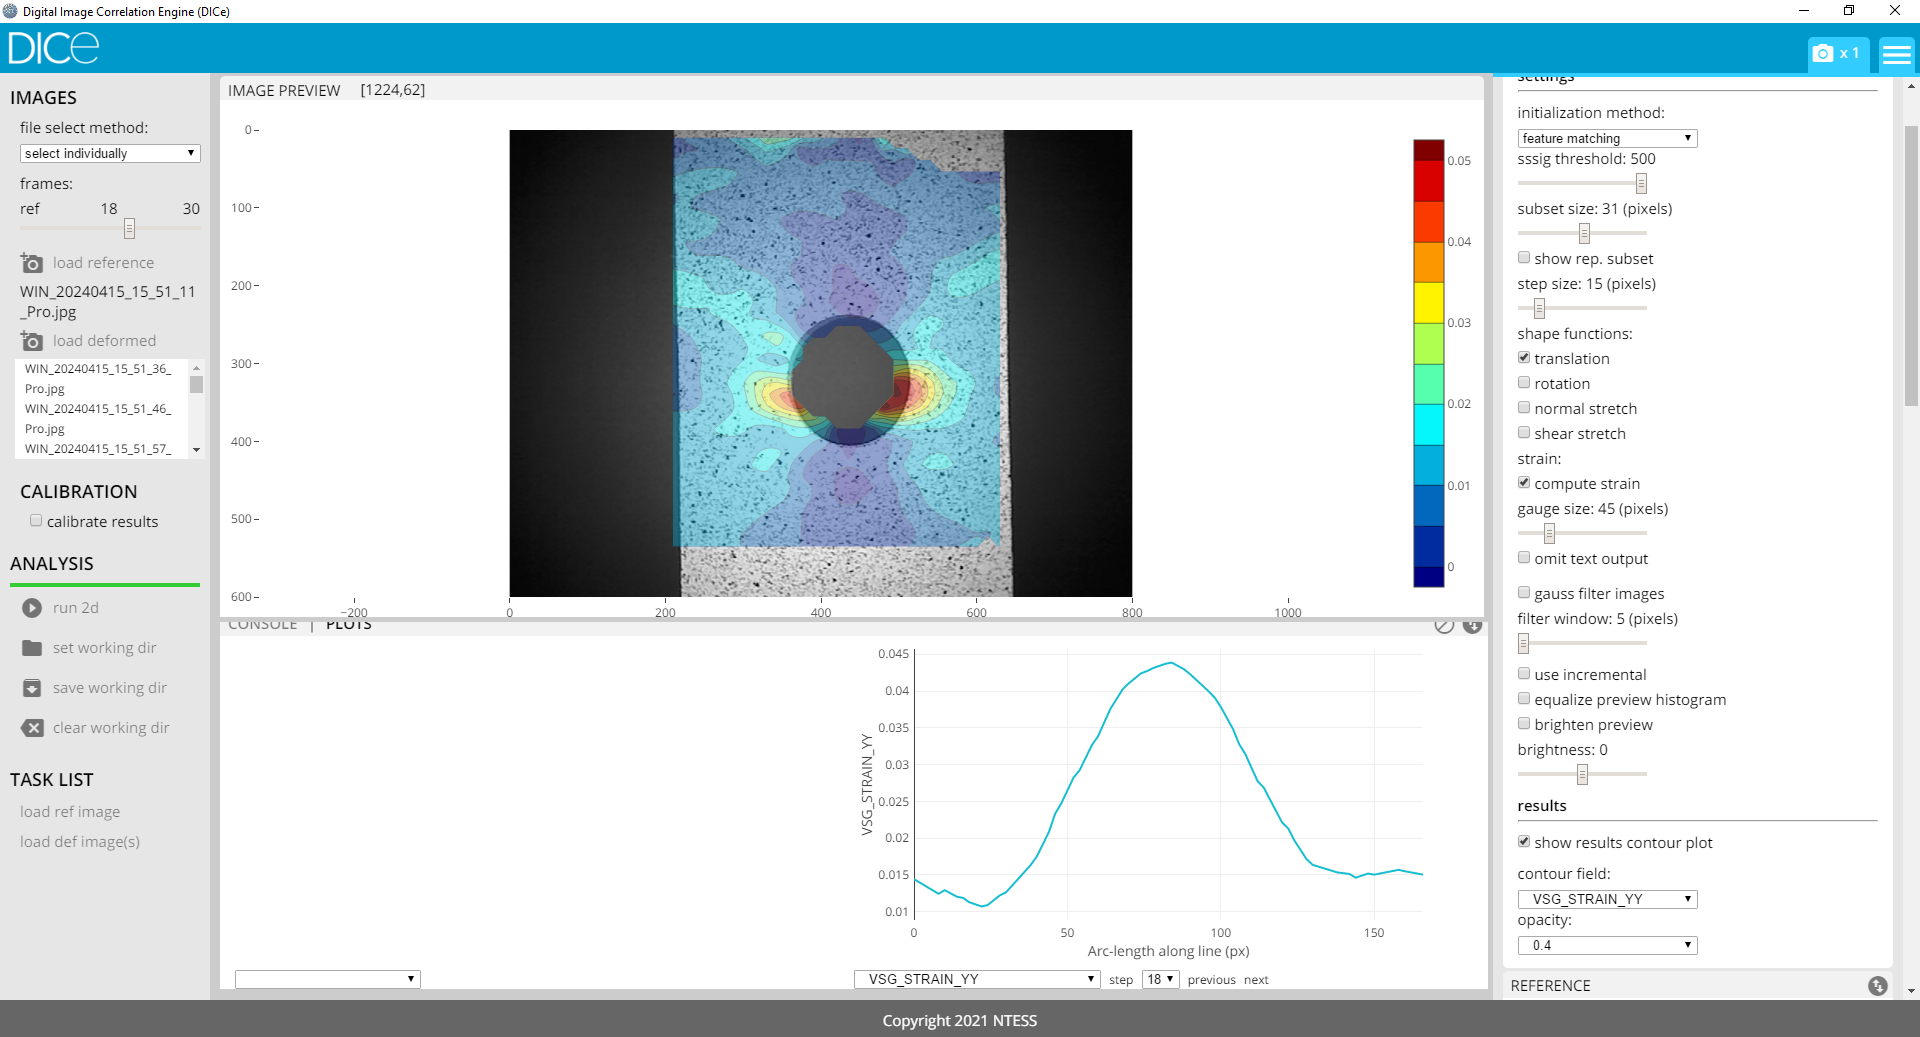
\includegraphics[width = 0.7\textwidth]{lab9images/DICE_software_page.PNG}
    \caption{DICe UI}
    \label{fig:dice}
\end{figure}

\item Load in the reference image (before tensile loading). Then load in the sequence of images after the reference once the strip begins to deform.

\item Use the line tool to draw a vertical line on the reference image as close to the edge of the center hole as possible. This will output a plot once the 2D images are analyzed.

\item On the right side panel, set the contour field to VSG\_STRAIN\_YY. Now on the left side panel, select 'run 2d'.
\begin{itemize}
    \item NOTE: Increasing the SSIG threshold may help with the analysis. The SSIG threshold was set to the max for our analysis.
\end{itemize}

 \item Run through the sequence of images analyzed with the 'frames' slider. There will be a plot of the strain distribution along the line drawn from earlier. 

 \item For each test article, select a good image and plot that represents the strain distribution around the center hole.

 \item This concludes the procedure. Processing this data and comparing to the theoretical values is next.

\end{enumerate}
\hypertarget{datapro}{}
\section{Data Processing}
\subsection{Variables and Equations}  

Nominal Stress at a cross-section containing the hole diameter:
\begin{equation}
    \sigma_{\text{nom}} = \dfrac{P}{t(D-d)}
\end{equation}

Variables:
\begin{itemize}
    \item \(P\): Applied tensile load
    \item \(t\): Thickness of test strip
    \item \(D\): Width of the test strip
    \item \(d\): Center hole diameter
\end{itemize}
\vspace{5mm}

Stress Concentration factor:
\begin{equation}
    K_{t} = \dfrac{\sigma_{\text{max}}}{\sigma_{\text{nom}}}
\end{equation}

Variables:
\begin{itemize}
    \item \(\sigma_{\text{max}}\): Maximum stress
\end{itemize}
\vspace{5mm}

Theoretical Stress Concentration factor (for $0 \leq d \leq D$):
\begin{equation}
    K_{t} = 3 - \pi\left(\dfrac{d}{D}\right) + \frac{11}{3}\left(\dfrac{d}{D}\right)^{2} - 1.527\left(\dfrac{d}{D}\right)^{3} 
\end{equation}
\vspace{5mm}

\begin{table}[H]
    \centering
    \begin{tabular}{c c c}
        \hline
        \hline 
        
         & Aluminum 7075-T6 & Poly-carbonate  \\  
         
         \hline
         
        Elastic Modulus & 71.7 GPa (10,400 ksi) & Avg. 2 GPa (290 ksi) \\[2pt]
        Yield Strength & 503 MPa (73 ksi) & 62.0 MPa (8.99 ksi) \\[2pt]
        Approx. Yield Strain & 0.7\% & 7.0\% \\[2pt]
        Poissons Ratio & 0.33 & 0.37 \\[2pt]
        
        \hline
        \hline
    \end{tabular}
    \caption{Material Properties of Test Articles}
    \label{tab:materialproperties}
\end{table}


\section{Results and Analysis}

%-----------------------------------------------------------------%
%Organize images of the aluminum and polycarbonate in this section%
%-----------------------------------------------------------------%

\begin{figure}[H]
    \centering
    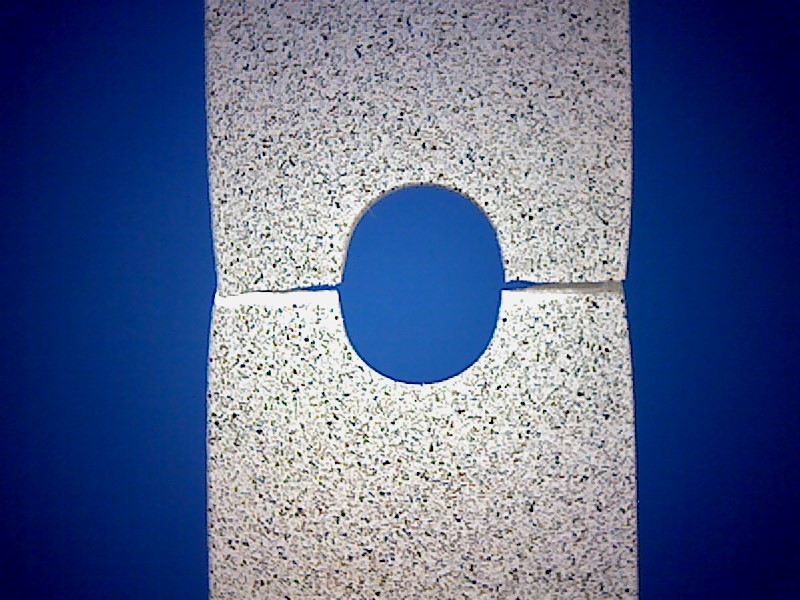
\includegraphics[width = 0.6\textwidth]{lab9images/aluminum_break.jpg}
    \caption{Aluminum at breakage}
    \label{fig:alfail}
\end{figure}

\begin{figure}[H]
    \centering
    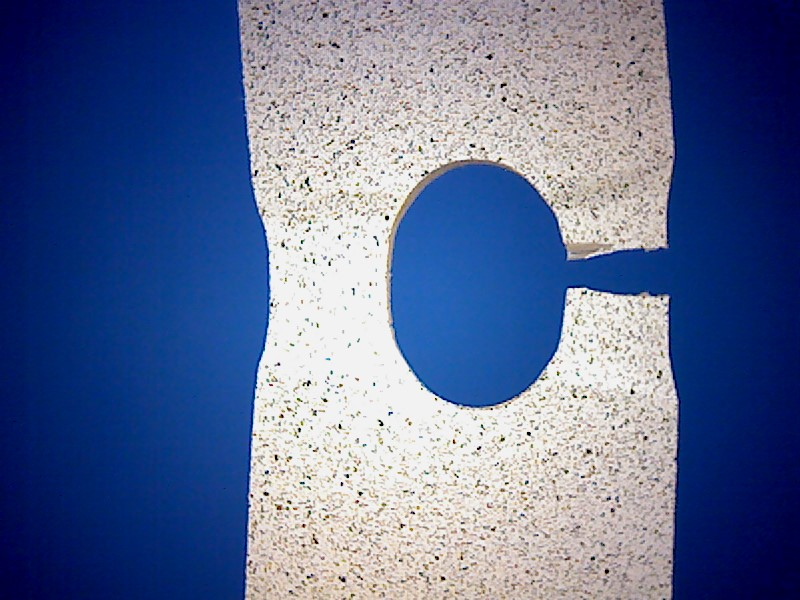
\includegraphics[width = 0.6\textwidth]{lab9images/polycarbonate_break.jpg}
    \caption{Poly-carbonate at breakage}
    \label{fig:PCfail}
\end{figure}

\begin{figure}[H]
    \centering
    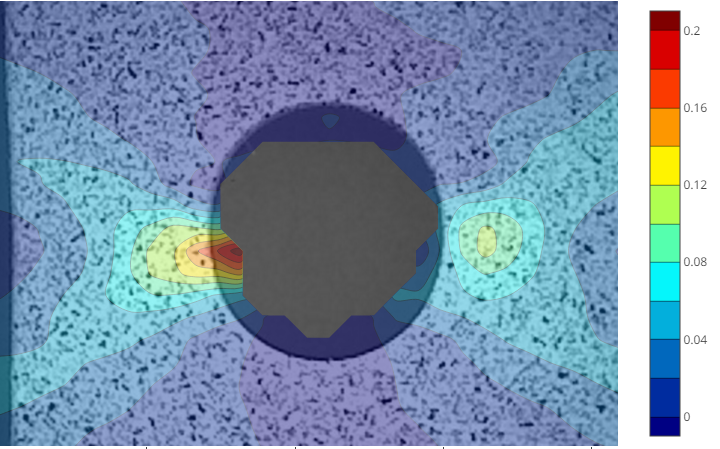
\includegraphics[width = 0.6\textwidth]{lab9images/meow color plot aluminum.PNG}
    \caption{Aluminum strain distribution image at 8kN}
    \label{fig:al8kNpic}
\end{figure}

\begin{figure}[H]
    \centering
    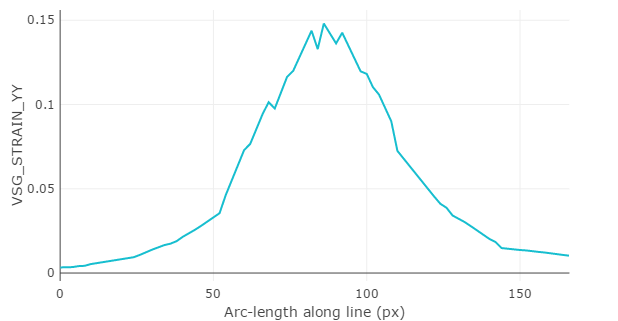
\includegraphics[width = 0.6\textwidth]{lab9images/8kNplot_Al_strainyy.png}
    \caption{Aluminum strain distribution plot at 8kN}
    \label{fig:al8kNplot}
\end{figure}

\begin{figure}[H]
    \centering
    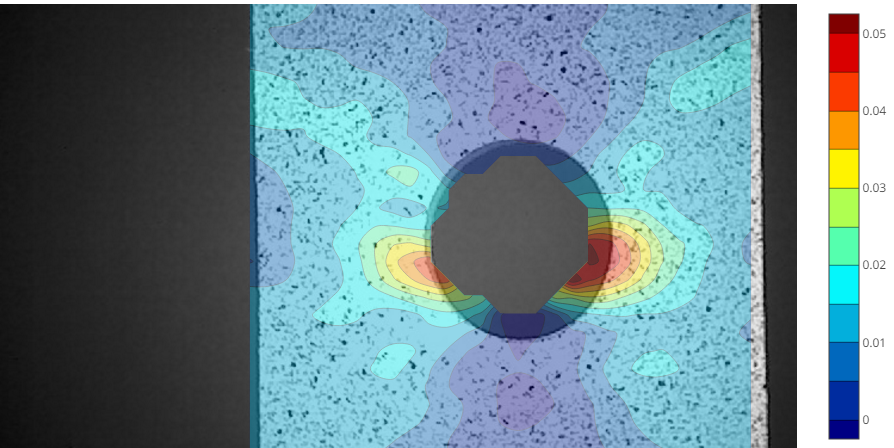
\includegraphics[width = 0.6\textwidth]{lab9images/1800Npccolored_strainyy.PNG}
    \caption{Poly-carbonate strain distribution image at 1800N}
    \label{fig:PC1800Npic}
\end{figure}

\begin{figure}[H]
    \centering
    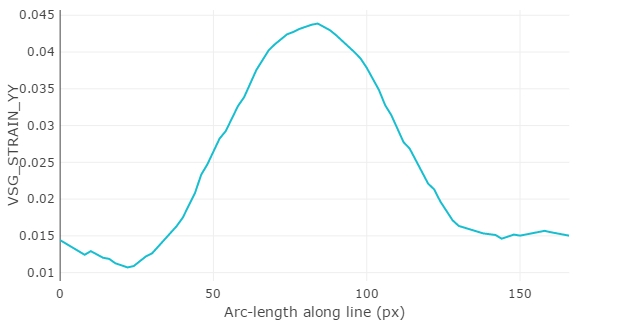
\includegraphics[width = 0.6\textwidth]{lab9images/1800Npcplot_strainyy.png}
    \caption{Poly-carbonate strain distribution plot at 1800N}
    \label{fig:PC1800Nplot}
\end{figure}
 
\section{Conclusion}



\newpage
\thispagestyle{empty}  % Clear header/footer
\begin{center}
	\vspace*{\fill}
	{\Huge Appendix}
	\vspace*{\fill}
\end{center}

% Start appendices
\newpage
\begin{appendices}
\pagestyle{fancy}
\renewcommand{\thefigure}{A\arabic{figure}}
\setcounter{figure}{0}

\pagebreak

\hypertarget{datasheets}{}
\section{Datasheets}
\begin{enumerate}[label = {[\arabic*]}]
\small
\item \hypertarget{1}{\href{https://www.instron.com/en/products/testing-systems/universal-testing-systems/low-force-universal-testing-systems/3300-series}{Instron 3300 Series Table Operator UTM}}
\item \hypertarget{2}{\href{https://www.sandia.gov/ccr/software/digital-image-correlation-engine-dice/}{Digital Image Correlation Engine (DICe) Software}}


\end{enumerate}

\end{appendices}

\end{document}
